\documentclass[25pt, a0paper, portrait, margin=0mm, innermargin=20mm,
blockverticalspace=2mm, colspace=20mm, subcolspace=0mm]{tikzposter} %Default values for poster format options.

\input{packages}

\definecolor{unired}{HTML}{a51e37}
\definecolor{mypink1}{rgb}{0.858, 0.188, 0.478}
\definecolor{mblack}{HTML}{0d0d0d}
\definecolor{titlecolor}{RGB}{74, 114, 159}
\definecolor{titledarkcolor}{RGB}{51,102,153}
\definecolor{Grey}{HTML}{e1e1e1}
\definecolor{DarkerGrey}{RGB}{215,217,219}
\definecolor{FontColor}{HTML}{0d0d0d}
\definecolor{Red}{RGB}{204,0,0}
\definecolor{L-lig}{RGB}{25,124,192}
\definecolor{point-lig}{RGB}{255,255,255}
\definecolor{G-lig}{RGB}{62,66,68}

\definecolor{Orange}{RGB}{240,163,10} 
\definecolor{LightRed}{RGB}{214,98,93}
\definecolor{LightBlue}{RGB}{160,200,217}
\definecolor{LightGreen}{RGB}{130,161,119}
\definecolor{Violet}{RGB}{190,144,252}

\colorlet{blocktitlefgcolor}{mblack}
\colorlet{backgroundcolor}{Grey}
\colorlet{blocktitlebgcolor}{Grey}
\colorlet{blockbodyfgcolor}{FontColor}
\colorlet{innerblocktitlebgcolor}{L-lig}
\colorlet{innerblocktitlefgcolor}{white}
\colorlet{notefrcolor}{white}
\colorlet{notefgcolor}{black}
\colorlet{notebgcolor}{white}




\begin{document}
 
\renewcommand{\baselinestretch}{1} 
\title{\parbox{1500pt}{Color-blindness of direction-selective units in the optic tectum}}
\author{Alexander Wendt, Patrick Weygoldt}
\institute{Systems Neurobiology, Department of Neurobiology, University of Tuebingen}
\usetitlestyle[]{sampletitle}
\maketitle
\renewcommand{\baselinestretch}{1.4} 

\begin{columns}
\column{0.3333}
\myblock[MyBlock]{Introduction}{
   Color has a big influence on motion vision in zebrafish. 
   Orger and Baier (2004) displayed with the optomotor response of zebrafish that motion blindness can be indueced 
   to a grating of different colors. 
   
   But little is known about the cortical structures conveing the
   \glqq color-motion\grqq{} perception. We wanted to the investigate the 
   optic tectum of the zebrafish larvae with calcium imaging. 
}
\myblock[MyBlock]{Preprocessing:}{
    \textbf{1. Region of Interests (ROI):}
    corrosponds to neurons with genetically. The lumiance $F$ of the calcium imaging is calculated from the change of luminance normalized to the average luminance $F = \frac{\Delta F}{F}$.
    
    \vspace{-2cm}
    \begin{tikzfigure}[]
        \label{Raw}
        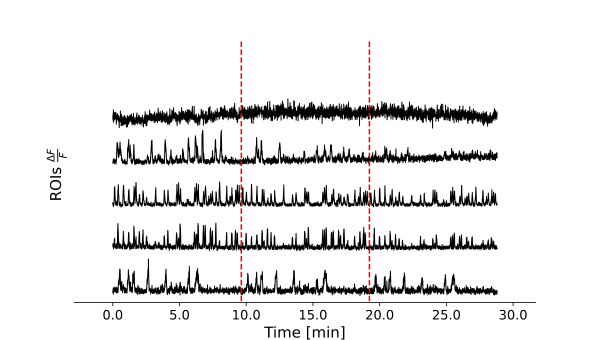
\includegraphics[width=24cm]{figs/autocorrelation.pdf}
    \end{tikzfigure} 
    \vspace{0.6cm}
    \textbf{2. Active ROIs:}
    To get the active ROIs we computed the correlation within 3 repeats of the same stimulus.  
    \vspace{-2cm}
    \begin{tikzfigure}[]
        \label{Rois}
        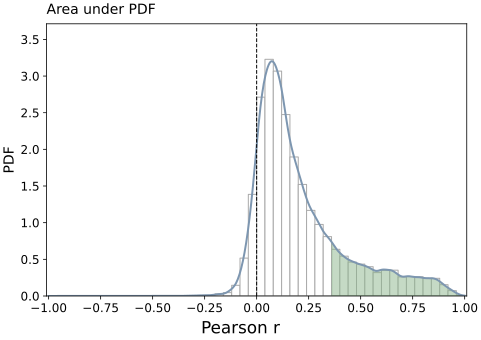
\includegraphics[width=12cm]{figs/pcorrelation.pdf}
    \end{tikzfigure} 
    \vspace{0.5}

    \textbf{2. Direction selective ROIs:} next Step was 
    to search for ROIs that correlated with a direction selective regressor (1 for clockwise = CW or counterclockwise = CCW, else is 0).
    
    \vspace{-0.7cm}
    \begin{tikzfigure}[]
        \label{Rois}
        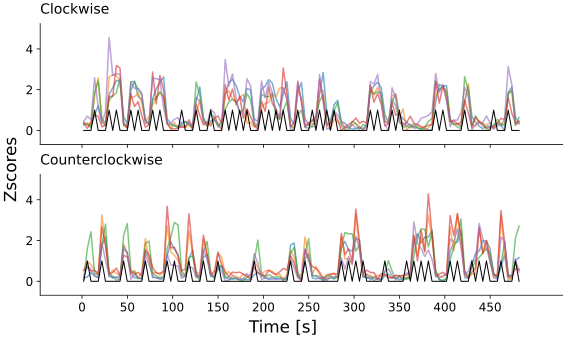
\includegraphics[width=24cm]{figs/regressor.pdf}
    \end{tikzfigure} 
    }

\column{0.6666}
\myblock[MyBlock]{2-photon calcium imaging}{
    \begin{tikzfigure}[]
        \label{modulations}
        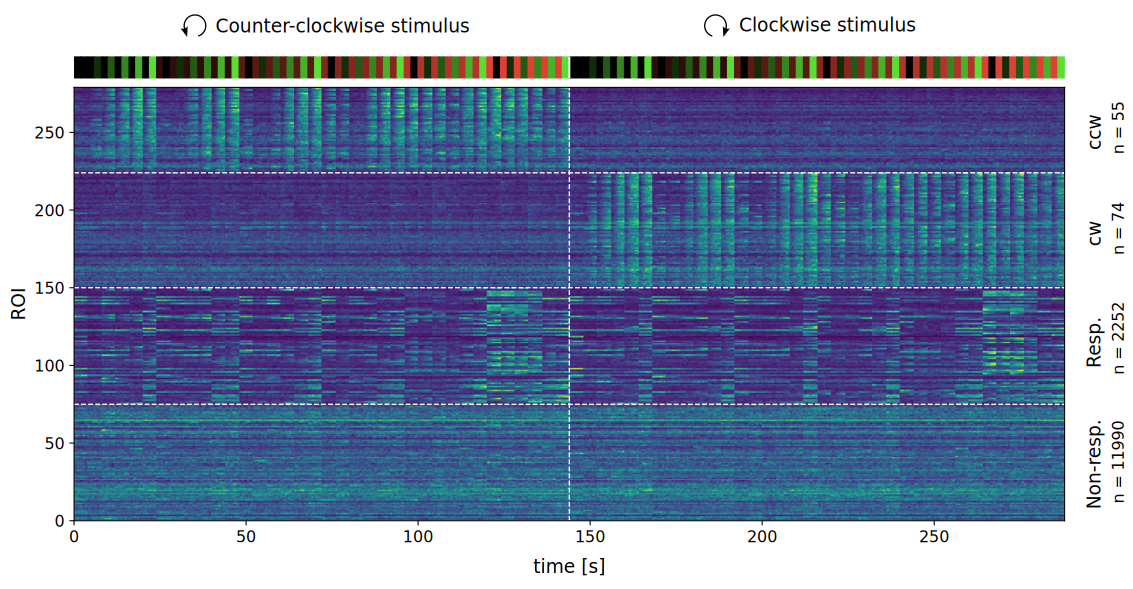
\includegraphics[width=\linewidth]{figs/testimg.pdf
        }
    \end{tikzfigure}

    \begin{tikzfigure}[]
        \label{Raw}
        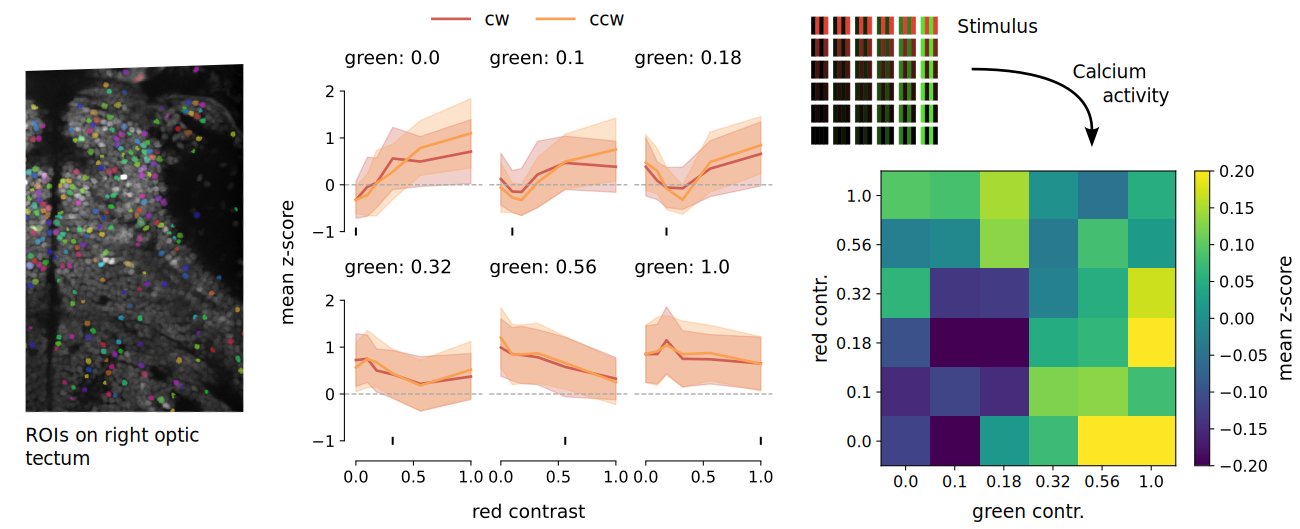
\includegraphics[width=50cm]{figs/contrast_curves_ca.pdf}
    \end{tikzfigure}
}

\myblock[MyBlock]{Behavior}{
    \begin{tikzfigure}[]
        \label{Raw}
        \includegraphics[width=50cm]{figs/contrast_curves_behav.pdf}
    \end{tikzfigure}

}
\myblock[MyBlock]{Conclusion}{
    \begin{itemize}
        \setlength\itemsep{0.5cm}
        \item The optic tectum is mottion blind for various contrast levels 
        
    \end{itemize}
    \vspace{0.2cm}
    }
\end{columns}

%\node [above right, text=white, outer sep=45pt,minimum width=\paperwidth, align=center, draw, fill=unired, color=unired] at (-43.6,-61) { \textcolor{white}{\normalsize Contact: patrick.weygoldt@student.uni-tuebingen.de}};

\end{document}